\section{Causalidade}

\begin{frame}{Causalidade}
    \begin{itemize}
        \item Causalidade é a relação entre causa e efeito;
        \item Aplicações relevantes na vida real: medicina, economia, política, etc.;
        \item Interesse crescente na área de pesquisa: Airbnb, Uber, Salesforce, Microsoft...
    \end{itemize}
    \vspace{20pt}
    Adotar o estudo de causalidade permite melhorar a tomada de decisão, prever resultados de intervenções e entender relações complexas entre variáveis.
\end{frame}

\begin{frame}{Interventions e o operador \emph{do}}
    Pearl introduziu um framework formal para modelar intervenções:

    \begin{itemize}
        \item \bm{$P(Y \mid X)$} representa a probabilidade de $Y$ dado que observamos $X$;
        \item \bm{$P(Y \mid do(X))$} representa a probabilidade de $Y$ quando intervenimos para fixar $X$ em um valor específico;
    \end{itemize}

    \pause
    \begin{itemize}
        \item \bm{$P(Y \mid X)$} reflete correlações que podem resultar de múltiplos caminhos causais.
        \item \bm{$P(Y \mid do(X))$} isola o efeito causal de $X$ sobre $Y$ simulando uma intervenção que elimina influências causais à $X$.
    \end{itemize}
\end{frame}

\begin{frame}{Interventions e o operador \emph{do}}{Um exemplo...}
    \begin{itemize}
        \item \bm{$P(recuperou \mid {medicado})$} indica: \pause correlação, possivelmente confundida por fatores como idade, gravidade da doença, etc.;
        \pause
        \item \bm{$P(recuperou \mid do({medicado}))$} indica: \pause o efeito causal do remédio na recuperação, isolando o impacto de outros fatores.
    \end{itemize}

    \pause

    Podemos distinguir essas duas probabilidades coletando mais dados?
    \pause
    \centering
    
\includegraphics[width=0.3\textwidth]{figures/no.jpg}
\end{frame}
\begin{frame}{Hierarquia Causal e os limites de ML tradicional}
    \begin{center}
        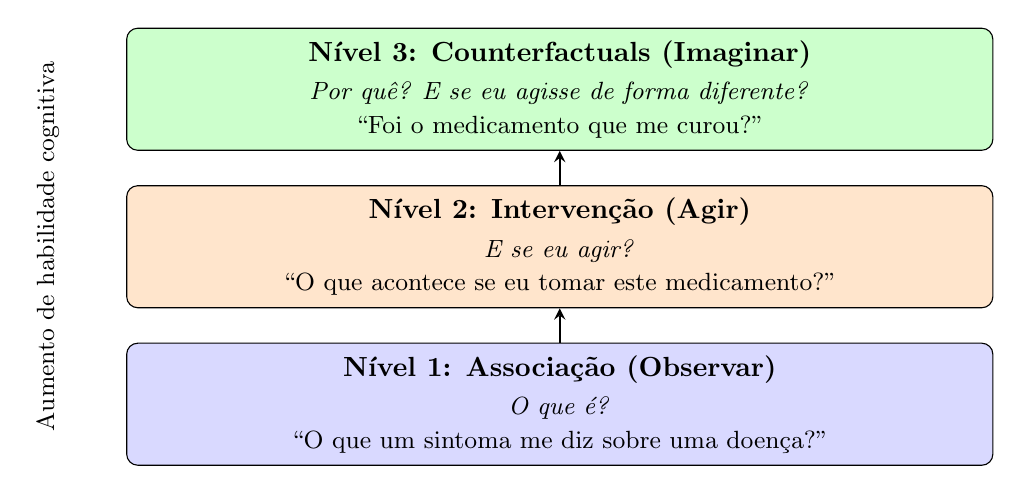
\begin{tikzpicture}[
            level/.style={draw, rounded corners, minimum width=11cm, minimum height=1.55cm, align=center},
            arrow/.style={->, thick, >=stealth}
        ]
        \node[level, fill=blue!15] (l1) at (0,0) {
            \textbf{Nível 1: Associação (Observar)} \\[2pt]
            \small \textit{O que é?} \\
            \small ``O que um sintoma me diz sobre uma doença?''
        };
        \node[level, fill=orange!20] (l2) at (0,2) {
            \textbf{Nível 2: Intervenção (Agir)} \\[2pt]
            \small \textit{E se eu agir?} \\
            \small ``O que acontece se eu tomar este medicamento?''
        };
        \node[level, fill=green!20] (l3) at (0,4) {
            \textbf{Nível 3: Counterfactuals (Imaginar)} \\[2pt]
            \small \textit{Por quê? E se eu agisse de forma diferente?} \\
            \small ``Foi o medicamento que me curou?''
        };
        \draw[arrow] (l1.north) -- (l2.south);
        \draw[arrow] (l2.north) -- (l3.south);
        \node[rotate=90, anchor=center] at (-6.5,2) {\small Aumento de habilidade cognitiva};
        \end{tikzpicture}
        \label{fig:causal_hierarchy}
    \end{center}
\end{frame}

\begin{frame}{Modelos Gráficos Causais}{Grafos Acíclicos Dirigidos (DAGs)}
    \begin{columns}[T]
        \begin{column}{0.52\textwidth}
            \begin{itemize}
                \item Nós = variáveis; 
                \item Arestas dirigidas = causalidade direta;
                \item $X \rightarrow Y$: $X$ é causa direta de $Y$ %($X$ é pai de $Y$)
                \vspace{20pt}
                \item<2-> Como esses grafos são "criados"?
                \item<3-> Modelados por especialistas de negócios...
                \item<4-> ...ou descobertos a partir de algoritmos especializados (Causal Discovery).
            \end{itemize}
        \end{column}
        \begin{column}{0.44\textwidth}
            \centering
            \vspace{6pt}
            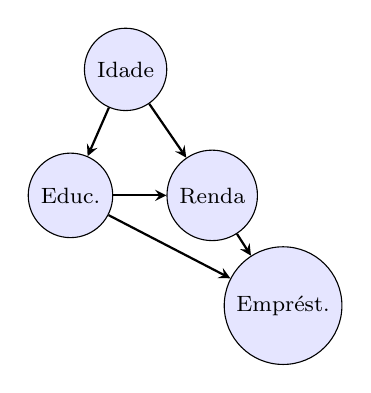
\begin{tikzpicture}[
                nd/.style={draw, circle, minimum size=0.9cm, fill=blue!10, font=\footnotesize},
                ar/.style={->, thick, >=stealth}
            ]
            \node[nd] (age)  at (1,   2)  {Idade};
            \node[nd] (edu)  at (0.3, 0.4) {Educ.};
            \node[nd] (inc)  at (2.1, 0.4) {Renda};
            \node[nd] (loan) at (3,  -1)   {Emprést.};
            \draw[ar] (age) -- (edu);
            \draw[ar] (age) -- (inc);
            \draw[ar] (edu) -- (inc);
            \draw[ar] (inc) -- (loan);
            \draw[ar] (edu) -- (loan);
            \end{tikzpicture}
            \label{fig:dag_example}
        \end{column}
    \end{columns}
\end{frame}

\begin{frame}{Modelos Gráficos Causais}{Confounders, Mediators e Colliders}
    Um \textit{confounder} é uma causa comum do tratamento \bm{$X$} e do resultado \bm{$Y$}, representado por uma bifurcação no DAG: \bm{$X \leftarrow Z \rightarrow Y$}.

    \bm{$Z$} cria uma associação espúria entre \bm{$X$} e \bm{$Y$}, mesmo que não haja relação causal direta entre eles.

    \vfill

    \begin{figure}[htbp]
        \centering
        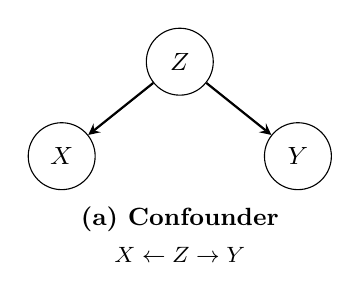
\begin{tikzpicture}[
            gnode/.style={draw, circle, minimum size=0.85cm, font=\small},
            arrow/.style={->, thick, >=stealth}
        ]
        % --- (a) Confounder (Fork) ---
        \node[gnode] (Xf) at (0.0, 0) {$X$};
        \node[gnode] (Zf) at (1.5, 1.2) {$Z$};
        \node[gnode] (Yf) at (3.0, 0) {$Y$};
        \draw[arrow] (Zf)--(Xf);
        \draw[arrow] (Zf)--(Yf);
        \node[font=\small\bfseries] at (1.5, -0.8) {(a) Confounder};
        \node[font=\footnotesize] at (1.5, -1.25) {$X \leftarrow Z \rightarrow Y$};
        \end{tikzpicture}
        \end{figure}
\end{frame}

\begin{frame}{Modelos Gráficos Causais}{Confounders, Mediators e Colliders}
    Um \textit{mediator} é uma variável que está no caminho causal entre \bm{$X$} e \bm{$Y$}, representado por uma cadeia no DAG: \bm{$X \rightarrow M \rightarrow Y$}.

    O mediador \bm{$M$} transmite o efeito causal de \bm{$X$} para \bm{$Y$}.

    \vfill

    \begin{figure}[htbp]
        \centering
        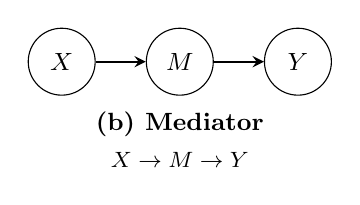
\begin{tikzpicture}[
            gnode/.style={draw, circle, minimum size=0.85cm, font=\small},
            arrow/.style={->, thick, >=stealth}
        ]
       
        % --- (b) Mediator (Chain) ---
        \node[gnode] (Xc) at (4.5, 0) {$X$};
        \node[gnode] (Mc) at (6.0, 0) {$M$};
        \node[gnode] (Yc) at (7.5, 0) {$Y$};
        \draw[arrow] (Xc)--(Mc);
        \draw[arrow] (Mc)--(Yc);
        \node[font=\small\bfseries] at (6.0, -0.8) {(b) Mediator};
        \node[font=\footnotesize] at (6.0, -1.25) {$X \rightarrow M \rightarrow Y$};

        \end{tikzpicture}
        \end{figure}
\end{frame}

\begin{frame}{Modelos Gráficos Causais}{Confounders, Mediators e Colliders}
    Um \textit{collider} é uma variável que é causada por outras duas variáveis, representado por uma estrutura em "V" no DAG: \bm{$X \rightarrow C \leftarrow Y$}.

    Diferente dos confounders e mediators, um collider não transmite associação entre \bm{$X$} e \bm{$Y$}, por padrão: \bm{$X$} e \bm{$Y$} são independentes, a menos que condicionemos em \bm{$C$} ou em um descendente de \bm{$C$}.

    \vfill

    \begin{figure}[htbp]
        \centering
        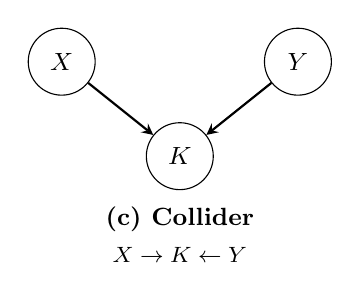
\begin{tikzpicture}[
            gnode/.style={draw, circle, minimum size=0.85cm, font=\small},
            arrow/.style={->, thick, >=stealth}
        ]

        % --- (c) Collider (V-structure) ---
        \node[gnode] (Xv) at (9.0, 1.2) {$X$};
        \node[gnode] (Kv) at (10.5, 0) {$K$};
        \node[gnode] (Yv) at (12.0, 1.2) {$Y$};
        \draw[arrow] (Xv)--(Kv);
        \draw[arrow] (Yv)--(Kv);
        \node[font=\small\bfseries] at (10.5, -0.8) {(c) Collider};
        \node[font=\footnotesize] at (10.5, -1.25) {$X \rightarrow K \leftarrow Y$};
        \end{tikzpicture}
        \end{figure}
\end{frame}

\begin{frame}{Modelos Gráficos Causais}{d-separation}
    \textit{Directional Separation (d-separation)} é um critério para determinar independência condicional em DAGs.

    Dois conjuntos de nós \bm{$X$} e \bm{$Y$} são d-separados por um conjunto de nós \bm{$Z$} se todas as trilhas entre \bm{$X$} e \bm{$Y$} forem bloqueadas por \bm{$Z$}.
    \vfill

    \begin{figure}[htbp]
        \centering
        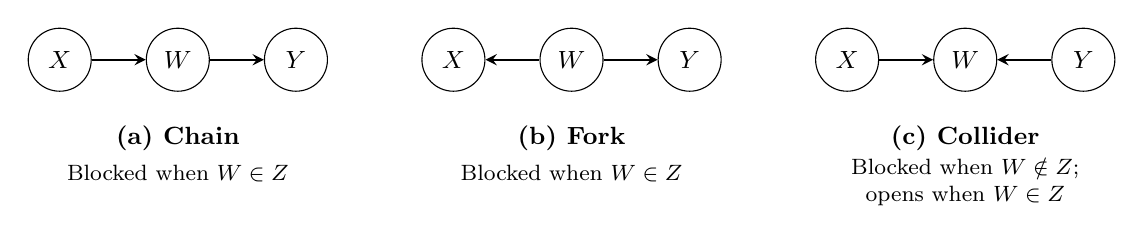
\begin{tikzpicture}[
            gnode/.style={draw, circle, minimum size=0.8cm, font=\small},
            arrow/.style={->, thick, >=stealth}
        ]
        % --- (a) Chain: X -> W -> Y ---
        \node[gnode] (X1) at (0.0, 0) {$X$};
        \node[gnode] (W1) at (1.5, 0) {$W$};
        \node[gnode] (Y1) at (3.0, 0) {$Y$};
        \draw[arrow] (X1)--(W1);
        \draw[arrow] (W1)--(Y1);
        \node[font=\small\bfseries] at (1.5, -1.0) {(a) Chain};
        \node[font=\footnotesize] at (1.5, -1.45) {Blocked when $W \in Z$};

        % --- (b) Fork: X <- W -> Y ---
        \node[gnode] (X2) at (5.0, 0) {$X$};
        \node[gnode] (W2) at (6.5, 0) {$W$};
        \node[gnode] (Y2) at (8.0, 0) {$Y$};
        \draw[arrow] (W2)--(X2);
        \draw[arrow] (W2)--(Y2);
        \node[font=\small\bfseries] at (6.5, -1.0) {(b) Fork};
        \node[font=\footnotesize] at (6.5, -1.45) {Blocked when $W \in Z$};

        % --- (c) Collider: X -> W <- Y ---
        \node[gnode] (X3) at (10.0, 0) {$X$};
        \node[gnode] (W3) at (11.5, 0) {$W$};
        \node[gnode] (Y3) at (13.0, 0) {$Y$};
        \draw[arrow] (X3)--(W3);
        \draw[arrow] (Y3)--(W3);
        \node[font=\small\bfseries] at (11.5, -1.0) {(c) Collider};
        \node[font=\footnotesize, align=center] at (11.5, -1.55) {Blocked when $W \notin Z$;\\opens when $W \in Z$};
        \end{tikzpicture}
        \end{figure}
\end{frame}

\begin{frame}{Modelos Gráficos Causais}{Equivalência de Markov}
    Múltiplos DAGs podem representar o mesmo conjunto de independências condicionais. Esses DAGs são chamados de \textit{Markov equivalent}.


    \begin{figure}
        \centering
	    
\includegraphics[width=0.65\linewidth]{figures/dags.jpg}
    \end{figure}
\end{frame}

\begin{frame}{Modelos Gráficos Causais}{Equivalência de Markov}
    \begin{itemize}
        \item[] \bm{$X \perp Z$}\ \ \ \ \ \ \ significa que \bm{$X$} é independente de \bm{$Z$}. 
        \item[] \bm{$X \perp Z \mid Y$} \ significa que \bm{$X$} é independente de \bm{$Z$} dado \bm{$Y$}. 
        \item[] \bm{$X \not\perp Z \mid Y$} \ significa que \bm{$X$} não é independente de \bm{$Z$} dado \bm{$Y$}.
    \end{itemize}
\end{frame}

\begin{frame}{Modelos Gráficos Causais}{Equivalência de Markov}
    \begin{figure}[htbp]
    \centering
    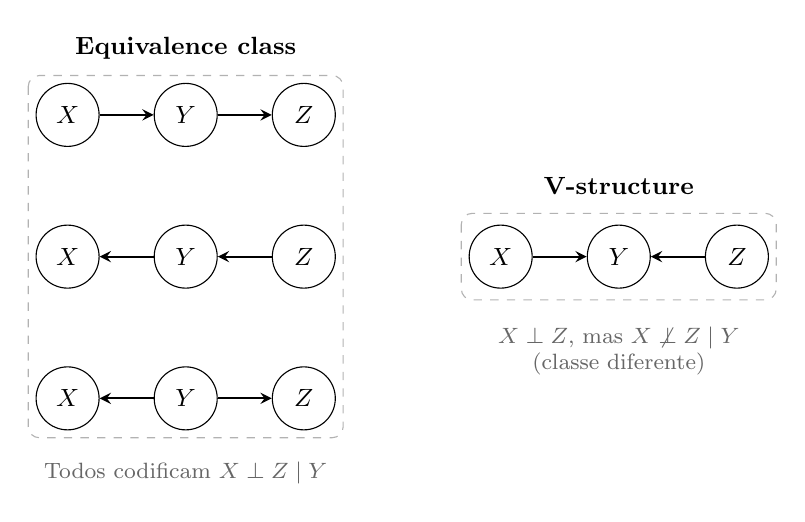
\begin{tikzpicture}[
        gnode/.style={draw, circle, minimum size=0.8cm, font=\small},
        arrow/.style={->, thick, >=stealth}
    ]
    % ---- Left column: three Markov-equivalent graphs ----
    % (a) X -> Y -> Z
    \node[gnode] (Xa) at (0.0,  0.0) {$X$};
    \node[gnode] (Ya) at (1.5,  0.0) {$Y$};
    \node[gnode] (Za) at (3.0,  0.0) {$Z$};
    \draw[arrow] (Xa)--(Ya); \draw[arrow] (Ya)--(Za);

    % (b) X <- Y <- Z
    \node[gnode] (Xb) at (0.0, -1.8) {$X$};
    \node[gnode] (Yb) at (1.5, -1.8) {$Y$};
    \node[gnode] (Zb) at (3.0, -1.8) {$Z$};
    \draw[arrow] (Yb)--(Xb); \draw[arrow] (Zb)--(Yb);

    % (c) X <- Y -> Z
    \node[gnode] (Xc) at (0.0, -3.6) {$X$};
    \node[gnode] (Yc) at (1.5, -3.6) {$Y$};
    \node[gnode] (Zc) at (3.0, -3.6) {$Z$};
    \draw[arrow] (Yc)--(Xc); \draw[arrow] (Yc)--(Zc);

    % Bounding box and label for the equivalence class
    \draw[dashed, rounded corners=4pt, gray!60] (-0.5, 0.5) rectangle (3.5, -4.1);
    \node[font=\small\bfseries] at (1.5,  0.85) {Equivalence class};
    \node[font=\footnotesize, gray!80!black] at (1.5, -4.55) {Todos codificam $X \perp Z \mid Y$};

    % ---- Right column: v-structure (different class) ----
    % (d) X -> Y <- Z
    \node[gnode] (Xd) at (5.5, -1.8) {$X$};
    \node[gnode] (Yd) at (7.0, -1.8) {$Y$};
    \node[gnode] (Zd) at (8.5, -1.8) {$Z$};
    \draw[arrow] (Xd)--(Yd); \draw[arrow] (Zd)--(Yd);

    % Bounding box and label for the v-structure
    \draw[dashed, rounded corners=4pt, gray!60] (5.0, -1.25) rectangle (9.0, -2.35);
    \node[font=\small\bfseries] at (7.0, -0.9) {V-structure};
    \node[font=\footnotesize, gray!80!black, align=center] at (7.0, -3.0) {$X \perp Z$, mas $X \not\perp Z \mid Y$\\(classe diferente)};

    \end{tikzpicture}
    \end{figure}
\end{frame}

\subsection{Outros modelos causais}

\begin{frame}{Outros modelos causais}{SCMs e Potential Outcomes}
    Dois frameworks algébricos complementam o modelo gráfico causal:
    \begin{itemize}
        \item \textbf{Structural Causal Models (SCMs)}, também de Pearl, descrevem relações causais usando equações estruturais, permitindo simulações e inferência causal;
        \item \textbf{Potential Outcomes}, de Rubin (também conhecido como \textit{Rubin Causal Model}) aborda causalidade na perspectiva de comparações de contrafactuais, sendo mais utilizado em estatística e ciências sociais.
    \end{itemize}

    \pause

    Os dois frameworks são complementares: SCMs fornece linguagem gráfica para codificar sobre a estrutura causal, e Potential Outcomes fornece estimandos e estratégias de estimativas causais.
\end{frame}

\begin{frame}{Efeitos causais}{Estimando efeitos causais}
    Para cada unidade \bm{$i$} e um valor de tratamento \bm{$t$}, existe um \texttt{resultado potencial} \bm{$Y_i(t)$}, que representa o resultado que seria observado se a unidade \bm{$i$} recebesse o tratamento \bm{$t$}.

    \vspace{20pt}
    \pause
    
    O efeito causal para a unidade \bm{$i$} é \bm{$\tau_i = Y_i(1) - Y_i(0)$}: a diferença entre o resultado potencial sob tratamento e o resultado potencial sob controle.
    
    \vspace{20pt}
    \pause

    No exemplo da vacinação, \bm{$Y_i(1)$} representa a probabilidade de recuperação se a pessoa for vacinada, e \bm{$Y_i(0)$} representa a probabilidade de recuperação se a pessoa não for vacinada.
\end{frame}
